% !TEX root=../report.tex

\section{Experiments}
\label{sec:experiment}

For this project, we trained our reinforcement learning models on 3 scenarios in the predator prey setting - 1) 1 green agent vs 1 red agent, 2) 2 green agents vs 1 red agent and 3) 1 green agent vs 2 red agents. We did not use any landmarks, as none of the algorithms we employ explicitly model the landmarks in their optimization, i.e., there is no constraint/penalty that prevents agents from attempting to "move through" the landmarks. Each of the 3 scenarios described above were performed with DQN, DDPG and MADDPG agents separately. The number of steps, collisions, average reward and average loss per episode were collected for all experiments. TODO: DQN vs MADDPG  

\subsection{1 Green Agent vs. 1 Red Agent}
\label{sec:experiment:1vs1}

Figure~\ref{fig:1vs1} plots our results for the predator-pray scenario with one
agent and one adversary. The first row of this figure shows the number of steps
per episode. The second row shows the cumulative reward per episode. The third
row shows the number of collisions per episode. The fourth row shows the
average loss per episode. The first column of Figure~\ref{fig:1vs1} shows the
results for DQN model. The second column shows the results for DDPG model. The
third column shows the results for MADDPG model. The x-axis of each figure is
always number of training episodes. We next analyze these results in turn.

\begin{figure}[t]
  \vspace*{-2cm}
  \begin{subfigure}[t]{\figscale\linewidth}
    \hspace*{-2.75cm}
    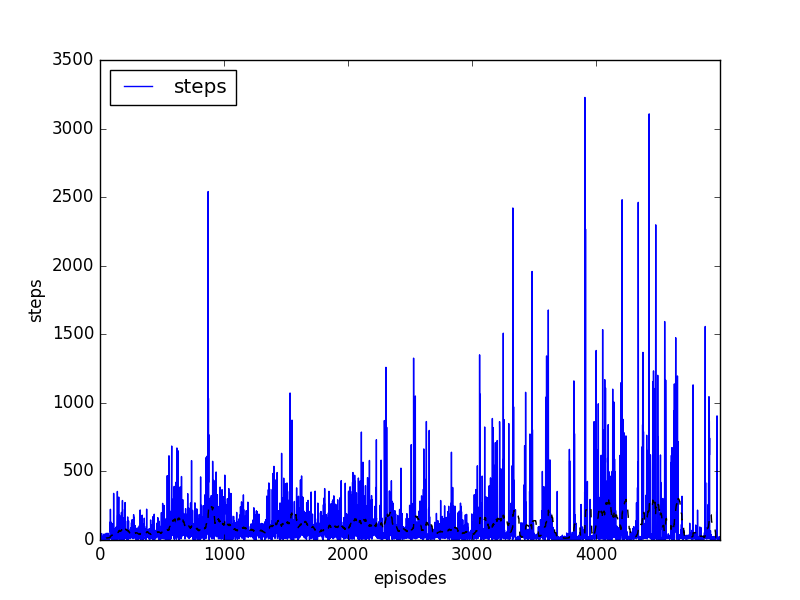
\includegraphics[width=1.5\textwidth]
    {../results/dqn_1vs1/steps.png}
    \label{fig:dqn-1vs1-steps}
  \end{subfigure}
  ~
  \begin{subfigure}[t]{\figscale\linewidth}
    \hspace*{-1.4cm}
    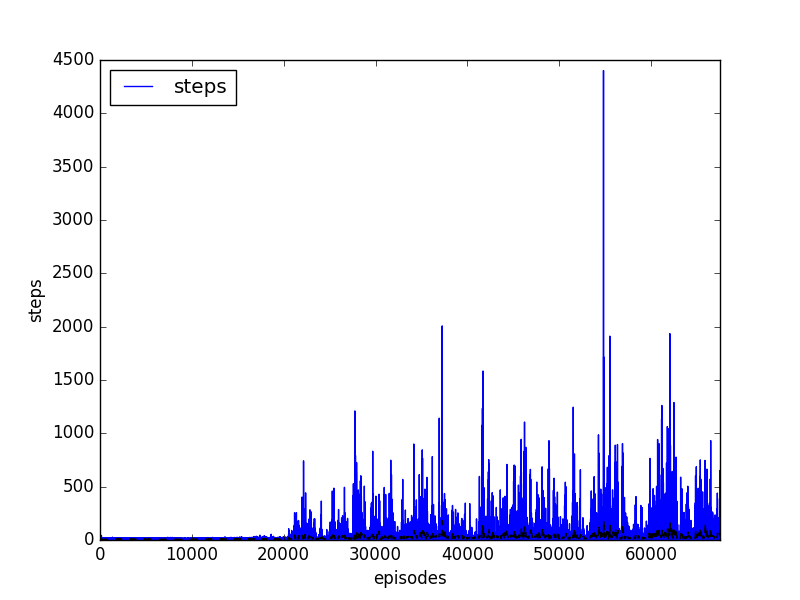
\includegraphics[width=1.5\textwidth]
    {../results/ddpg_1vs1/steps.png}
    \label{fig:ddpg-1vs1-steps}
  \end{subfigure}
  ~
  \begin{subfigure}[t]{\figscale\linewidth}
    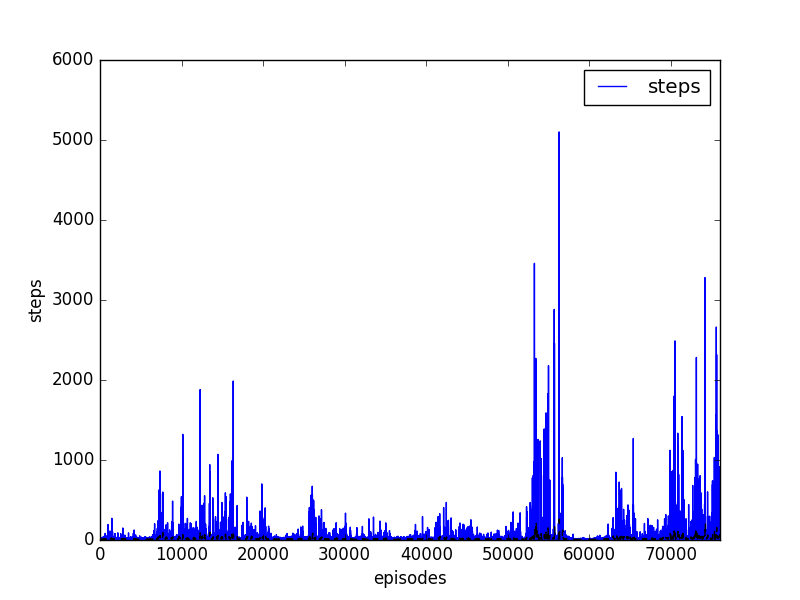
\includegraphics[width=1.5\textwidth]
    {../results/maddpg_1vs1/steps.png}
    \label{fig:maddpg-1vs1-steps}
  \end{subfigure}

  \vspace{-0.5cm}
  \begin{subfigure}[t]{\figscale\linewidth}
    \hspace*{-2.75cm}
    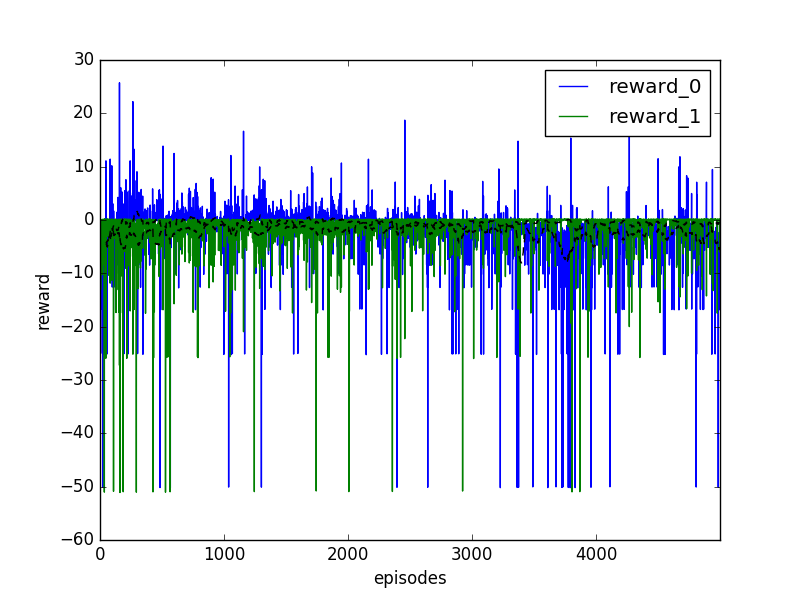
\includegraphics[width=1.5\textwidth]
    {../results/dqn_1vs1/reward.png}
    \label{fig:dqn-1vs1-reward}
  \end{subfigure}
  ~
  \begin{subfigure}[t]{\figscale\linewidth}
    \hspace*{-1.4cm}
    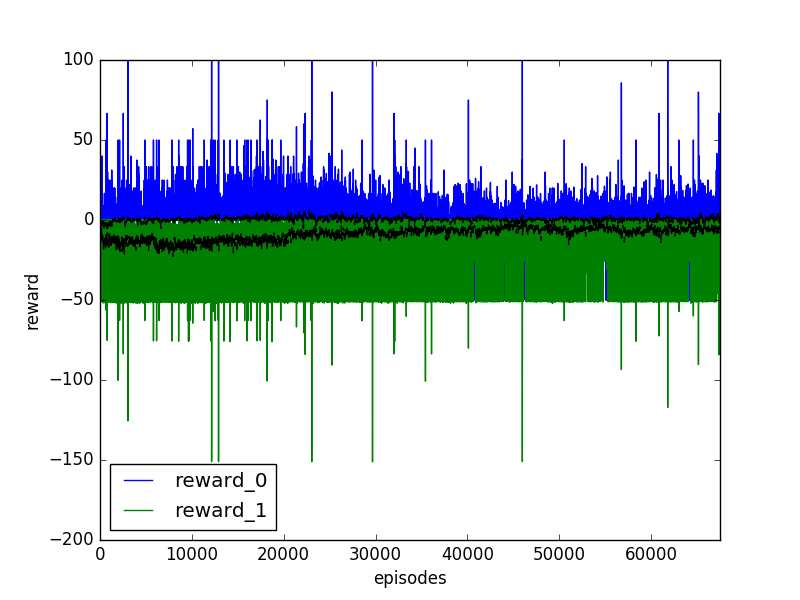
\includegraphics[width=1.5\textwidth]
    {../results/ddpg_1vs1/reward.png}
    \label{fig:ddpg-1vs1-reward}
  \end{subfigure}
  ~
  \begin{subfigure}[t]{\figscale\linewidth}
    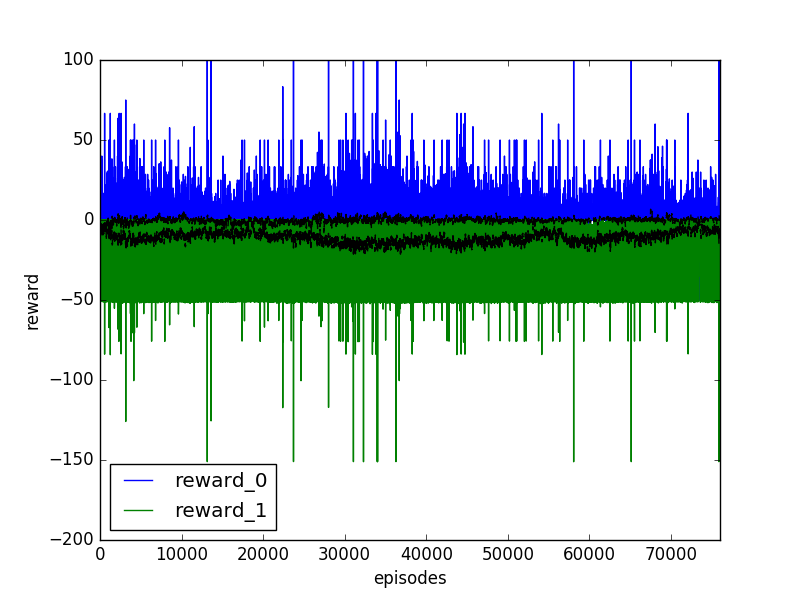
\includegraphics[width=1.5\textwidth]
    {../results/maddpg_1vs1/reward.png}
    \label{fig:maddpg-1vs1-reward}
  \end{subfigure}

  \vspace{-0.5cm}
  \begin{subfigure}[t]{\figscale\linewidth}
    \hspace*{-2.75cm}
    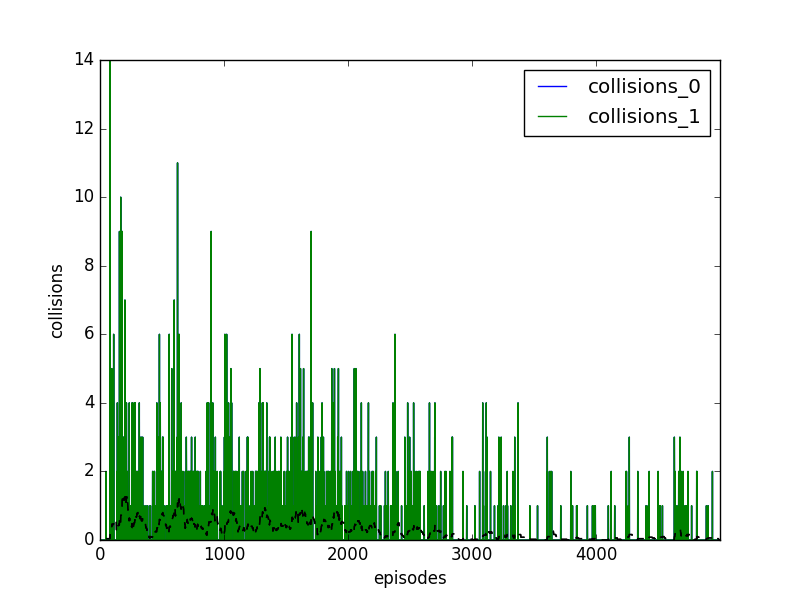
\includegraphics[width=1.5\textwidth]
    {../results/dqn_1vs1/collisions.png}
    \label{fig:dqn-1vs1-collisions}
  \end{subfigure}
  ~
  \begin{subfigure}[t]{\figscale\linewidth}
    \hspace*{-1.4cm}
    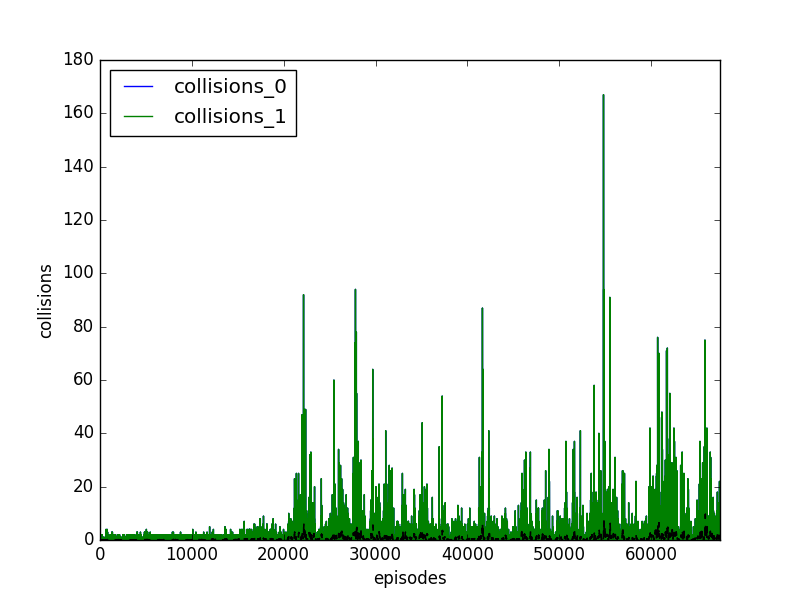
\includegraphics[width=1.5\textwidth]
    {../results/ddpg_1vs1/collisions.png}
    \label{fig:ddpg-1vs1-collisions}
  \end{subfigure}
  ~
  \begin{subfigure}[t]{\figscale\linewidth}
    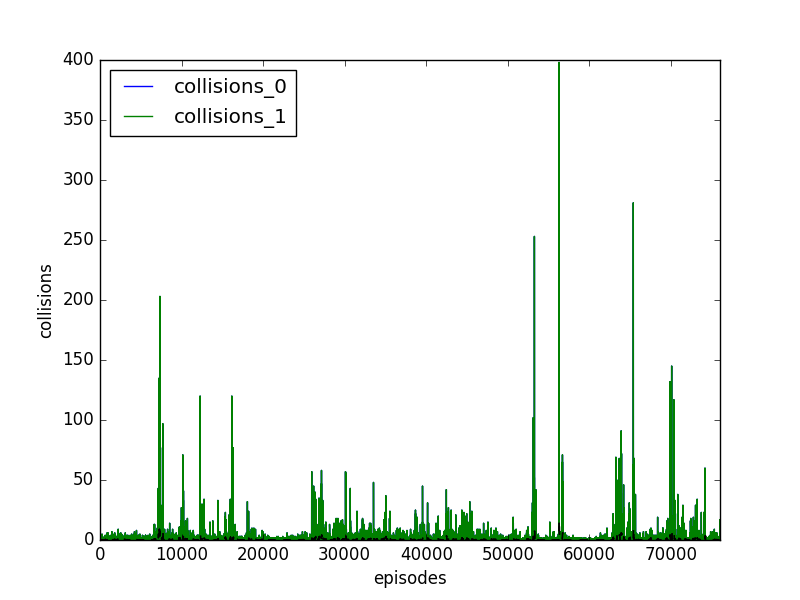
\includegraphics[width=1.5\textwidth]
    {../results/maddpg_1vs1/collisions.png}
    \label{fig:maddpg-1vs1-collisions}
  \end{subfigure}

  \vspace{-0.5cm}
  \begin{subfigure}[t]{\figscale\linewidth}
    \hspace*{-2.75cm}
    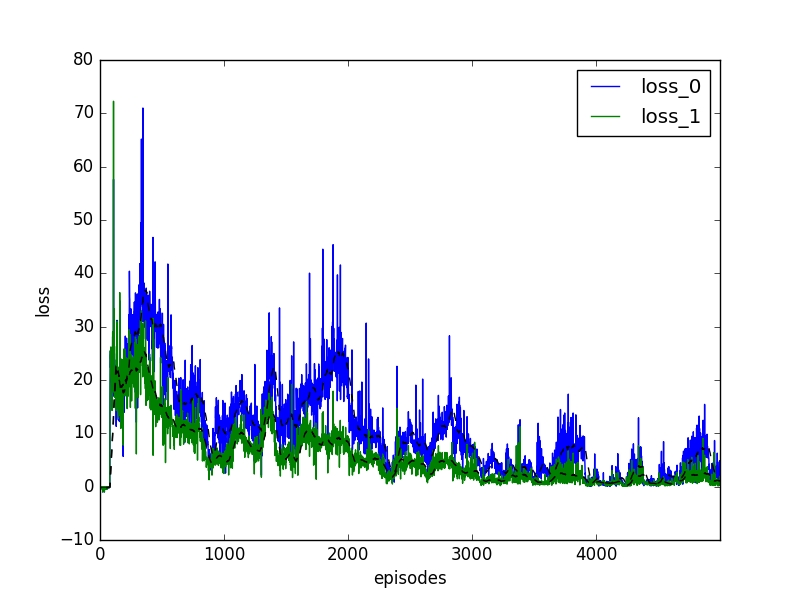
\includegraphics[width=1.5\textwidth]
    {../results/dqn_1vs1/loss.png}
    \label{fig:dqn-1vs1-loss}
  \end{subfigure}
  ~
  \begin{subfigure}[t]{\figscale\linewidth}
    \hspace*{-1.4cm}
    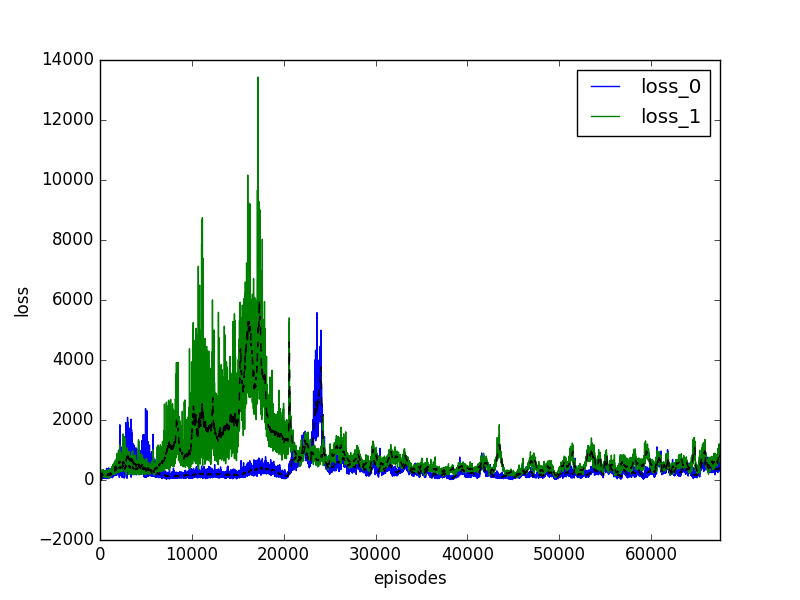
\includegraphics[width=1.5\textwidth]
    {../results/ddpg_1vs1/loss.png}
    \label{fig:ddpg-1vs1-loss}
  \end{subfigure}
  ~
  \begin{subfigure}[t]{\figscale\linewidth}
    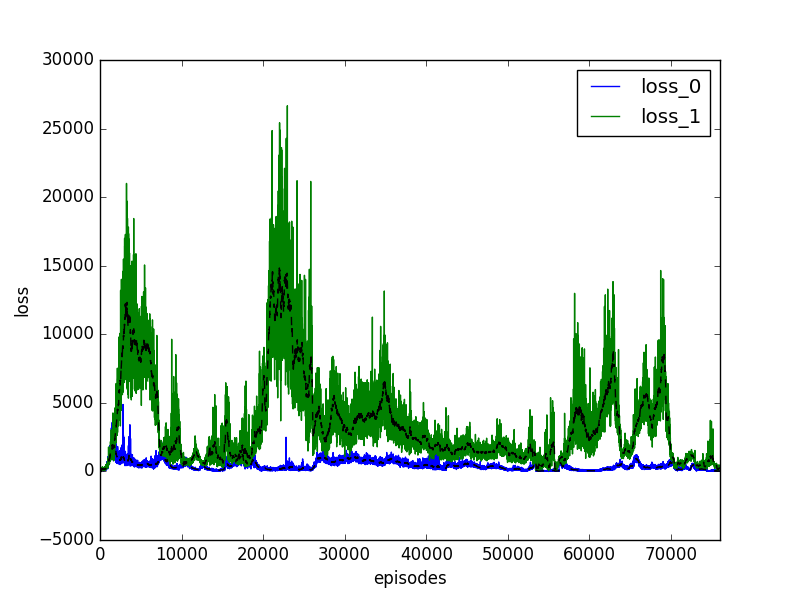
\includegraphics[width=1.5\textwidth]
    {../results/maddpg_1vs1/loss.png}
    \label{fig:maddpg-1vs1-loss}
  \end{subfigure}

  \caption{Plots for steps, average reward, collisions and loss per episode for 1 green vs 1 red agent. \textit{Left Column}: DQN, \textit{Middle Column}: DDPG, \textit{Right Column}: MADDPG}
  \label{fig:1vs1}
\end{figure}
\FloatBarrier

In the first row of Figure~\ref{fig:1vs1}, the blue curve shows the number of
steps for each episode, the black dotted curve shows the running average of
steps per episode with a window size of 50. Note the different y-axis scales
used in different figures. First, we observe that the MADDPG model achieves the
highest peak steps per episode of the three models (i.e., highest steps of
around 5000 achieved at around 55,000 episodes). Second, we find that DQN
achieves the highest average steps per episode of around 300. This shows that
DQN model based agent is has a more stable performance than the other two
models. This is likely because both DDPG and MADDPG use policy gradient method,
and uses a continuous action space rather than a discrete action space in DQN,
both of which make DDPG and MADDPG harder to train and less stable.

In the second row of Figure~\ref{fig:1vs1}, the blue curve shows the cumulative
episode reward for the red agent, and the green curve shows that for the green
adversary. Similar to the first row, we use black dotted curves to show the
running average of the episode rewards of each agent. Note that this is a zero
sum game because the rewards for collision and l2 distance should cancel out
each other. Only the reward for getting close to the boundary do not cancel
with each other. First, we observe that,
for DQN agent, the average episode reward increases quickly within 300
episodes and remain stable afterwards. Second, we find that the episode rewards
are more structured (i.e., most of the time the green adversary receives -50
rewards and the red agent receives near 50 rewards), whereas the rewards are
more random for the DQN agent (i.e., only a few episodes have high or low
rewards, mostly near zero rewards). Third, we find that the average reward for
DQN agent is higher than DDPG and MADDPG agents. This is because the DQN agent
is more stable and goes out of the screen less often.

In the third row of Figure~\ref{fig:1vs1}, the blue and green curves are
overlapped because the agent and the adversary have the same number of
collisions.

\subsection{2 Green Agents vs. 1 Red Agent}
\label{sec:experiment:1vs2}

\begin{figure}[t]
  \vspace*{-2cm}
  \begin{subfigure}[t]{\figscale\linewidth}
    \hspace*{-2.75cm}
    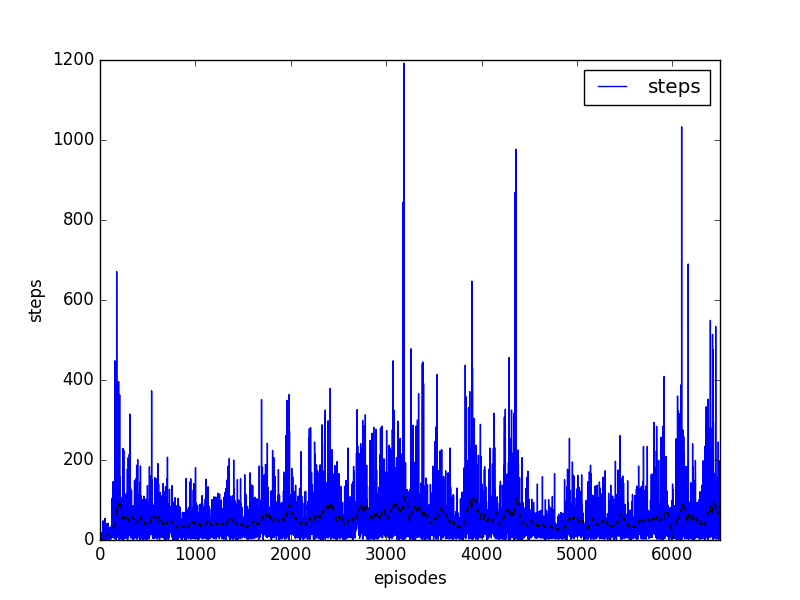
\includegraphics[width=1.5\textwidth]
    {../results/dqn_1vs2/steps.png}
    \label{fig:dqn-1vs2-steps}
  \end{subfigure}
  ~
  \begin{subfigure}[t]{\figscale\linewidth}
    \hspace*{-1.4cm}
    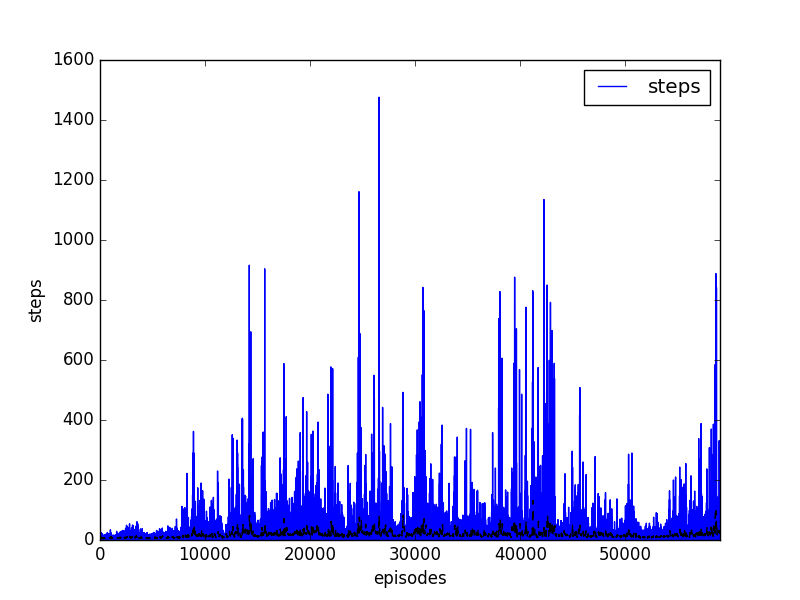
\includegraphics[width=1.5\textwidth]
    {../results/ddpg_1vs2/steps.png}
    \label{fig:ddpg-1vs2-steps}
  \end{subfigure}
  ~
  \begin{subfigure}[t]{\figscale\linewidth}
    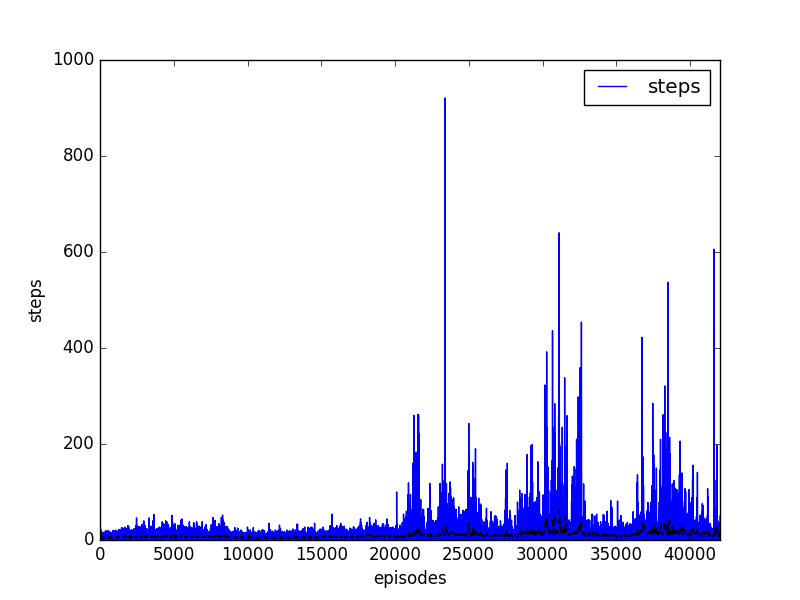
\includegraphics[width=1.5\textwidth]
    {../results/maddpg_1vs2/steps.png}
    \label{fig:maddpg-1vs2-steps}
  \end{subfigure}

  \vspace{-0.5cm}
  \begin{subfigure}[t]{\figscale\linewidth}
    \hspace*{-2.75cm}
    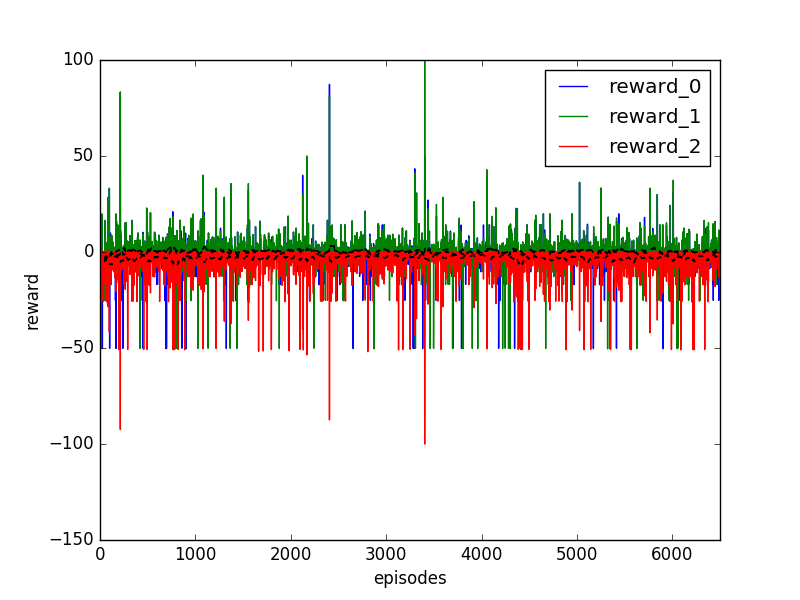
\includegraphics[width=1.5\textwidth]
    {../results/dqn_1vs2/reward.png}
    \label{fig:dqn-1vs2-reward}
  \end{subfigure}
  ~
  \begin{subfigure}[t]{\figscale\linewidth}
    \hspace*{-1.4cm}
    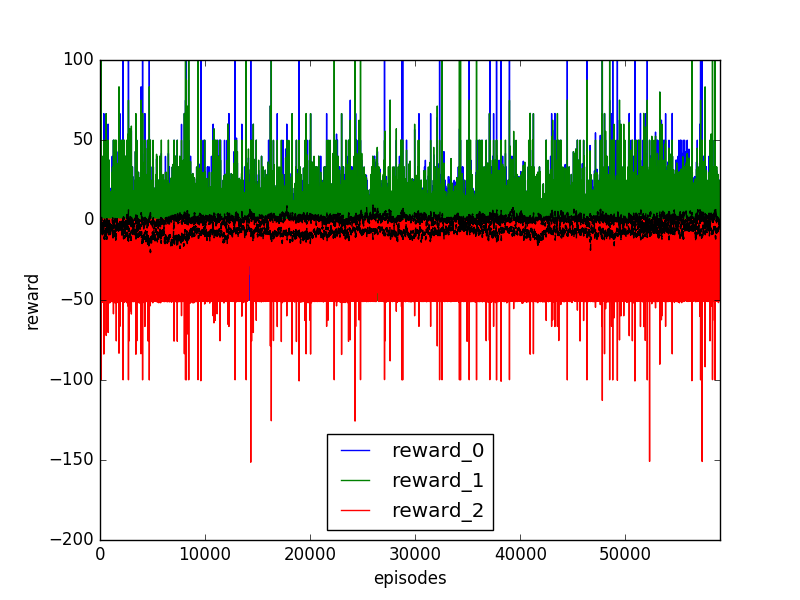
\includegraphics[width=1.5\textwidth]
    {../results/ddpg_1vs2/reward.png}
    \label{fig:ddpg-1vs2-reward}
  \end{subfigure}
  ~
  \begin{subfigure}[t]{\figscale\linewidth}
    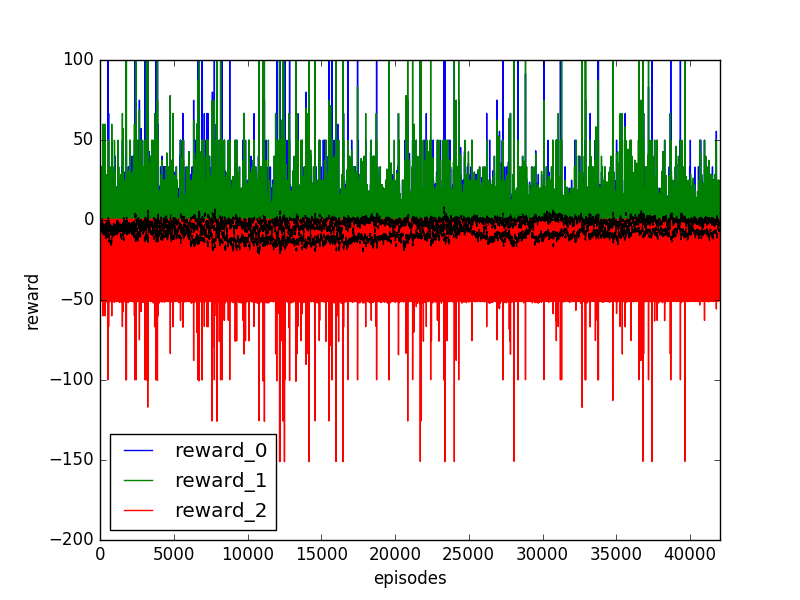
\includegraphics[width=1.5\textwidth]
    {../results/maddpg_1vs2/reward.png}
    \label{fig:maddpg-1vs2-reward}
  \end{subfigure}

  \vspace{-0.5cm}
  \begin{subfigure}[t]{\figscale\linewidth}
    \hspace*{-2.75cm}
    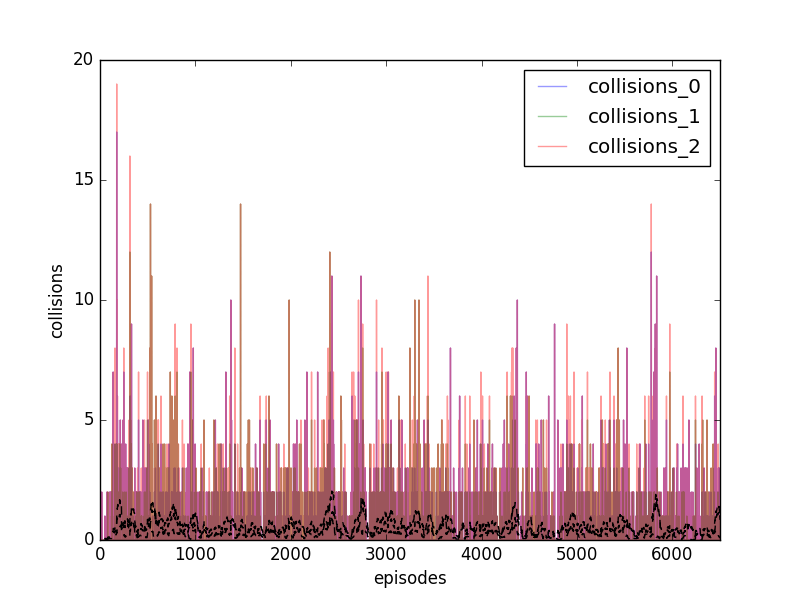
\includegraphics[width=1.5\textwidth]
    {../results/dqn_1vs2/collisions.png}
    \label{fig:dqn-1vs2-collisions}
  \end{subfigure}
  ~
  \begin{subfigure}[t]{\figscale\linewidth}
    \hspace*{-1.4cm}
    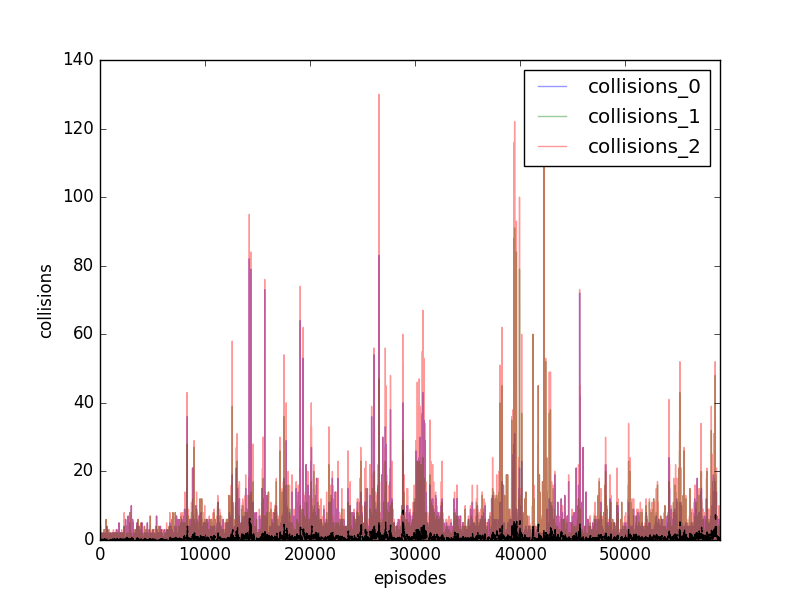
\includegraphics[width=1.5\textwidth]
    {../results/ddpg_1vs2/collisions.png}
    \label{fig:ddpg-1vs2-collisions}
  \end{subfigure}
  ~
  \begin{subfigure}[t]{\figscale\linewidth}
    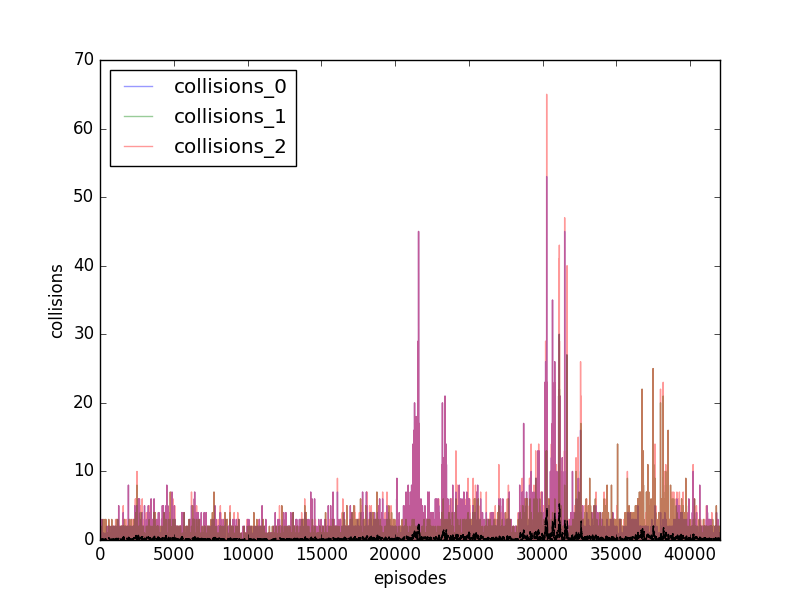
\includegraphics[width=1.5\textwidth]
    {../results/maddpg_1vs2/collisions.png}
    \label{fig:maddpg-1vs2-collisions}
  \end{subfigure}

  \vspace{-0.5cm}
  \begin{subfigure}[t]{\figscale\linewidth}
    \hspace*{-2.75cm}
    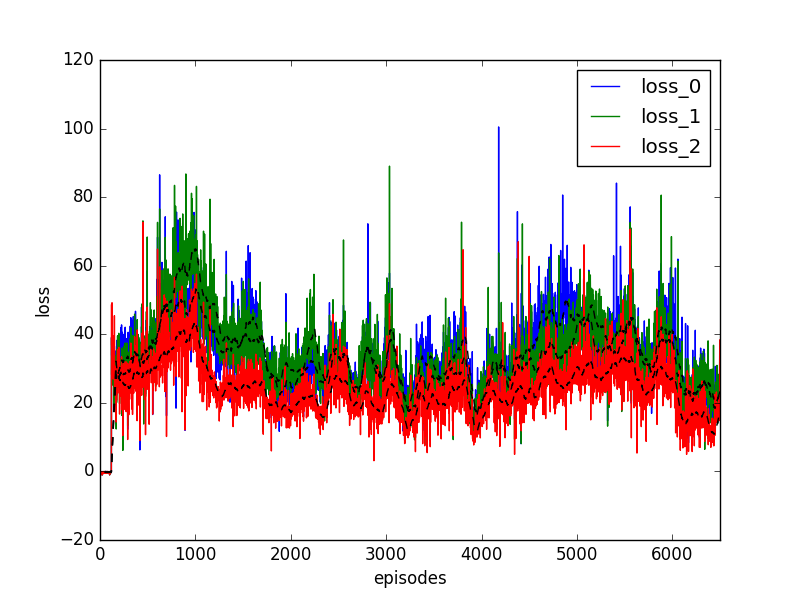
\includegraphics[width=1.5\textwidth]
    {../results/dqn_1vs2/loss.png}
    \label{fig:dqn-1vs2-loss}
  \end{subfigure}
  ~
  \begin{subfigure}[t]{\figscale\linewidth}
    \hspace*{-1.4cm}
    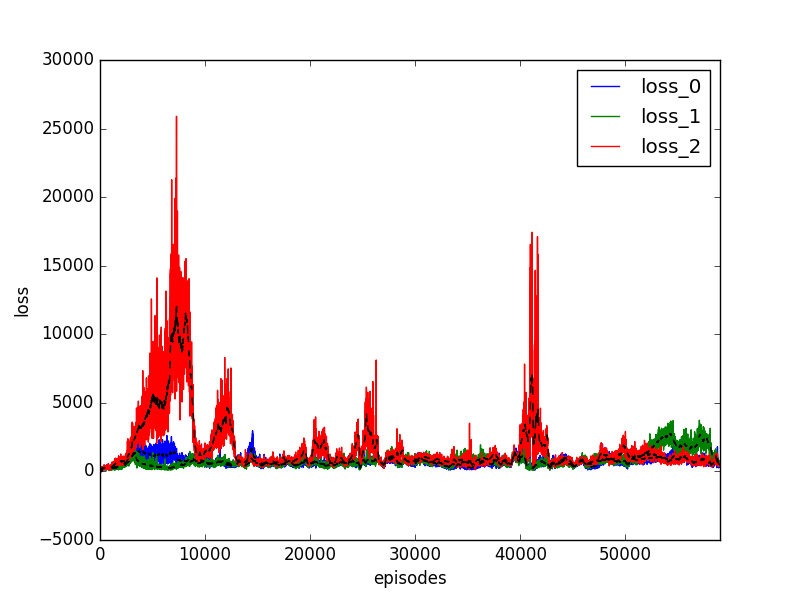
\includegraphics[width=1.5\textwidth]
    {../results/ddpg_1vs2/loss.png}
    \label{fig:ddpg-1vs2-loss}
  \end{subfigure}
  ~
  \begin{subfigure}[t]{\figscale\linewidth}
    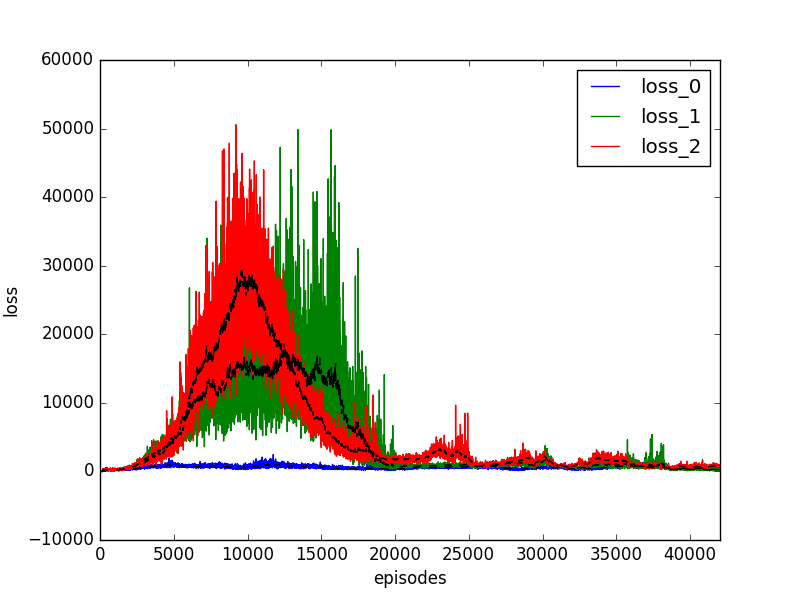
\includegraphics[width=1.5\textwidth]
    {../results/maddpg_1vs2/loss.png}
    \label{fig:maddpg-1vs2-loss}
  \end{subfigure}

  \caption{Plots for steps, average reward, collisions and loss per episode for 2 green vs 1 red agent. \textit{Left Column}: DQN, \textit{Middle Column}: DDPG, \textit{Right Column}: MADDPG}
  \label{fig:1vs2}
\end{figure}
\FloatBarrier

\subsection{1 Green Agent vs. 2 Red Agents}
\label{sec:experiment:2vs1}

\begin{figure}[t]
  \vspace*{-2cm}
  \begin{subfigure}[t]{\figscale\linewidth}
    \hspace*{-2.75cm}
    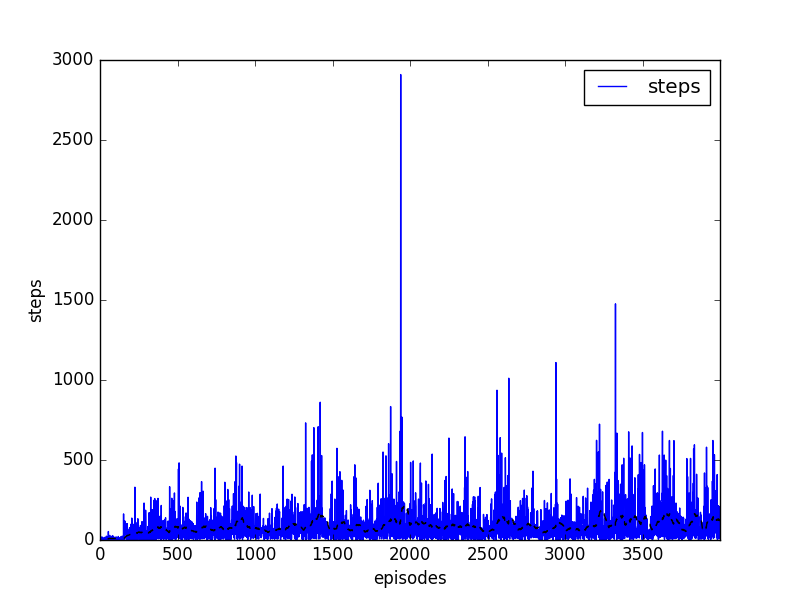
\includegraphics[width=1.5\textwidth]
    {../results/dqn_2vs1/steps.png}
    \label{fig:dqn-2vs1-steps}
  \end{subfigure}
  ~
  \begin{subfigure}[t]{\figscale\linewidth}
    \hspace*{-1.4cm}
    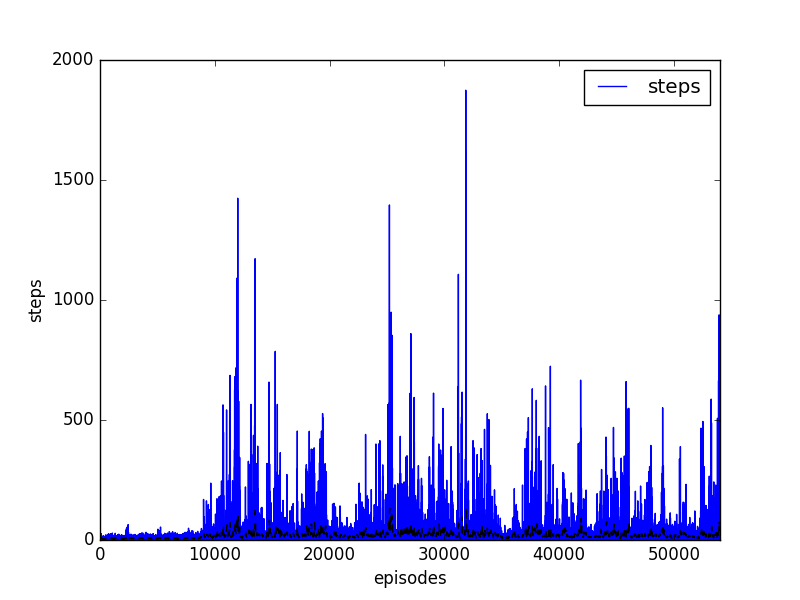
\includegraphics[width=1.5\textwidth]
    {../results/ddpg_2vs1/steps.png}
    \label{fig:ddpg-2vs1-steps}
  \end{subfigure}
  ~
  \begin{subfigure}[t]{\figscale\linewidth}
    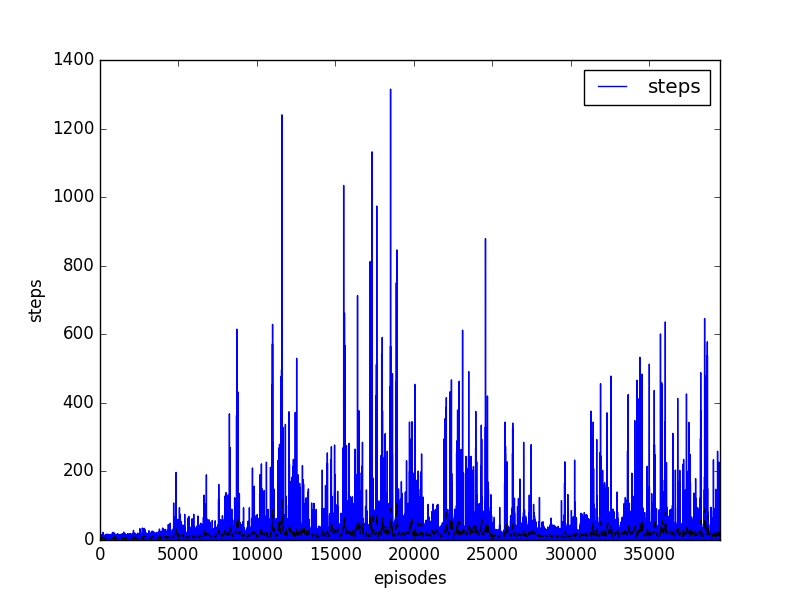
\includegraphics[width=1.5\textwidth]
    {../results/maddpg_2vs1/steps.png}
    \label{fig:maddpg-2vs1-steps}
  \end{subfigure}

  \vspace{-0.5cm}
  \begin{subfigure}[t]{\figscale\linewidth}
    \hspace*{-2.75cm}
    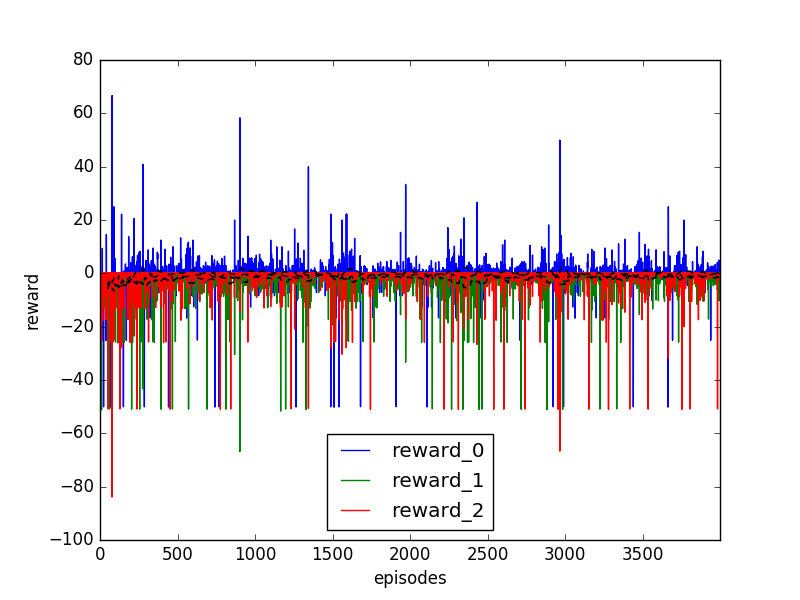
\includegraphics[width=1.5\textwidth]
    {../results/dqn_2vs1/reward.png}
    \label{fig:dqn-2vs1-reward}
  \end{subfigure}
  ~
  \begin{subfigure}[t]{\figscale\linewidth}
    \hspace*{-1.4cm}
    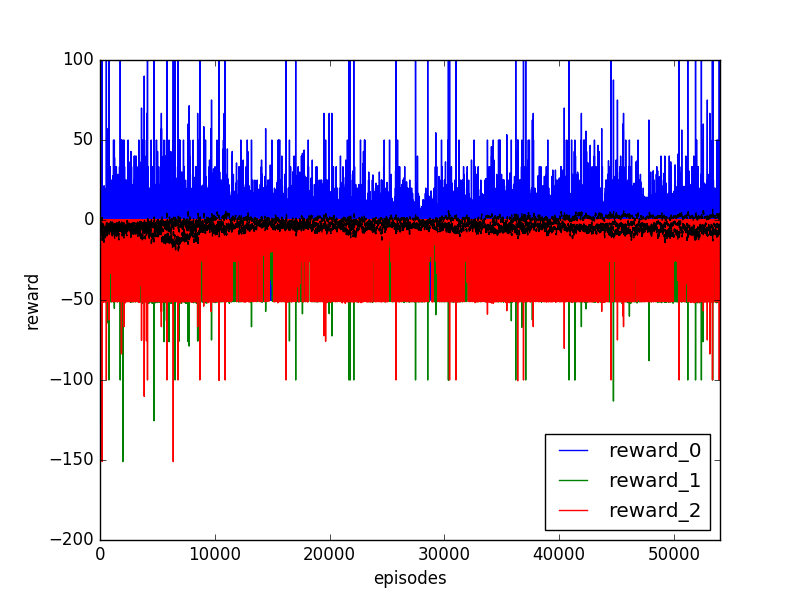
\includegraphics[width=1.5\textwidth]
    {../results/ddpg_2vs1/reward.png}
    \label{fig:ddpg-2vs1-reward}
  \end{subfigure}
  ~
  \begin{subfigure}[t]{\figscale\linewidth}
    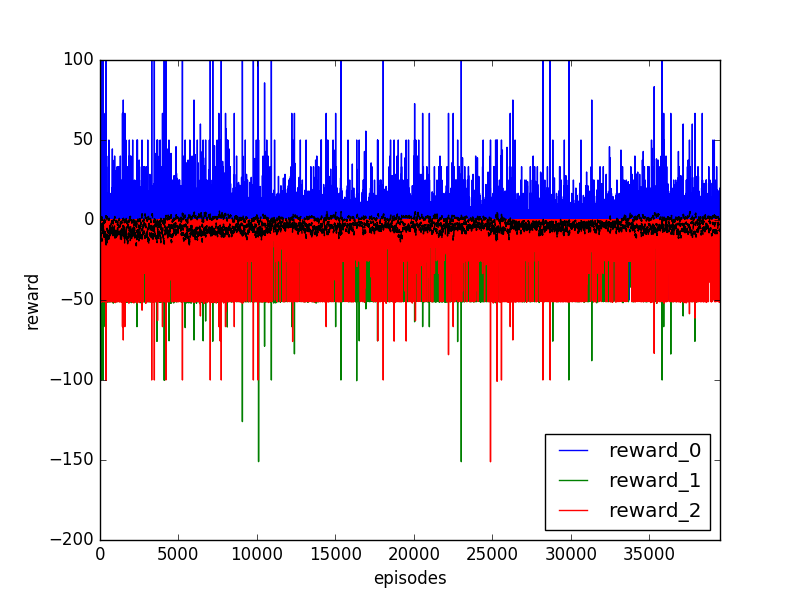
\includegraphics[width=1.5\textwidth]
    {../results/maddpg_2vs1/reward.png}
    \label{fig:maddpg-2vs1-reward}
  \end{subfigure}

  \vspace{-0.5cm}
  \begin{subfigure}[t]{\figscale\linewidth}
    \hspace*{-2.75cm}
    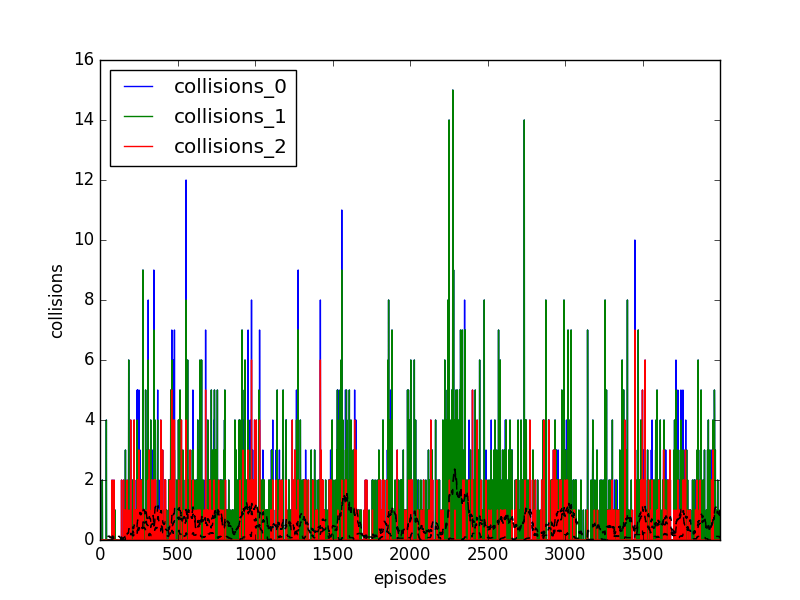
\includegraphics[width=1.5\textwidth]
    {../results/dqn_2vs1/collisions.png}
    \label{fig:dqn-2vs1-collisions}
  \end{subfigure}
  ~
  \begin{subfigure}[t]{\figscale\linewidth}
    \hspace*{-1.4cm}
    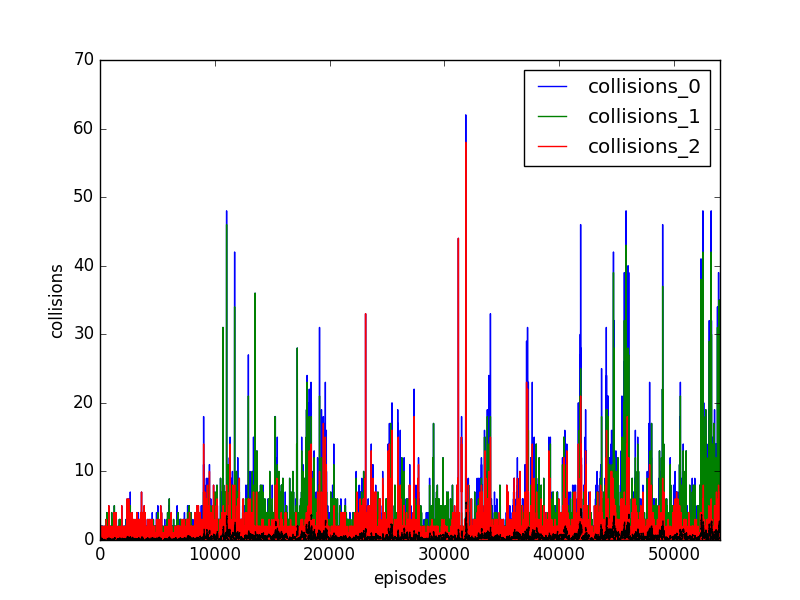
\includegraphics[width=1.5\textwidth]
    {../results/ddpg_2vs1/collisions.png}
    \label{fig:ddpg-2vs1-collisions}
  \end{subfigure}
  ~
  \begin{subfigure}[t]{\figscale\linewidth}
    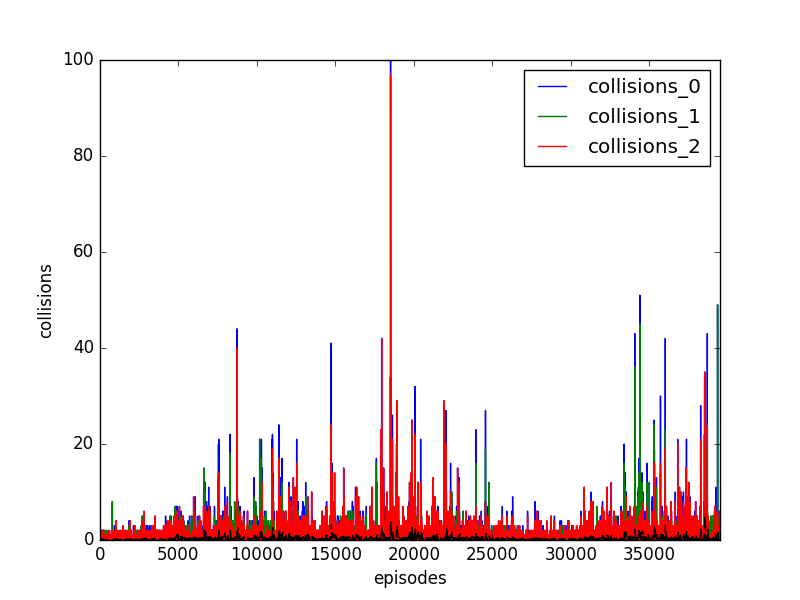
\includegraphics[width=1.5\textwidth]
    {../results/maddpg_2vs1/collisions.png}
    \label{fig:maddpg-2vs1-collisions}
  \end{subfigure}

  \vspace{-0.5cm}
  \begin{subfigure}[t]{\figscale\linewidth}
    \hspace*{-2.75cm}
    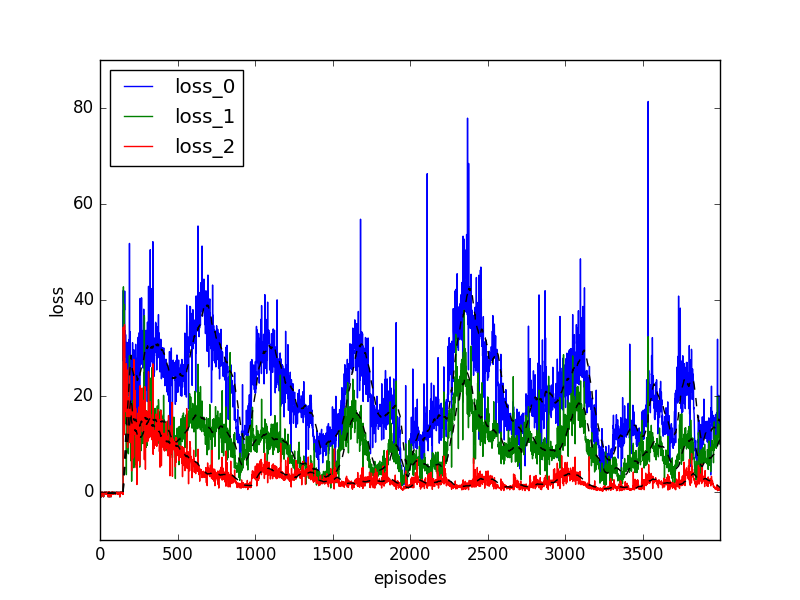
\includegraphics[width=1.5\textwidth]
    {../results/dqn_2vs1/loss.png}
    \label{fig:dqn-2vs1-loss}
  \end{subfigure}
  ~
  \begin{subfigure}[t]{\figscale\linewidth}
    \hspace*{-1.4cm}
    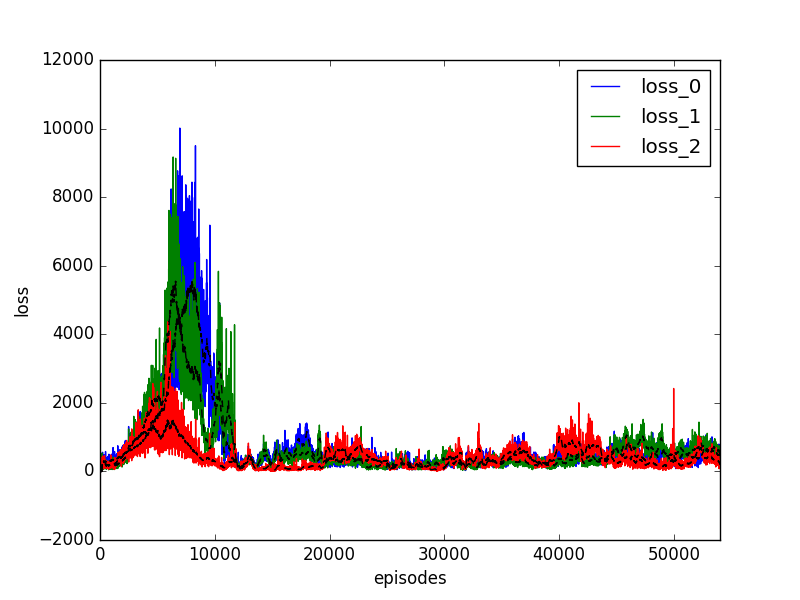
\includegraphics[width=1.5\textwidth]
    {../results/ddpg_2vs1/loss.png}
    \label{fig:ddpg-2vs1-loss}
  \end{subfigure}
  ~
  \begin{subfigure}[t]{\figscale\linewidth}
    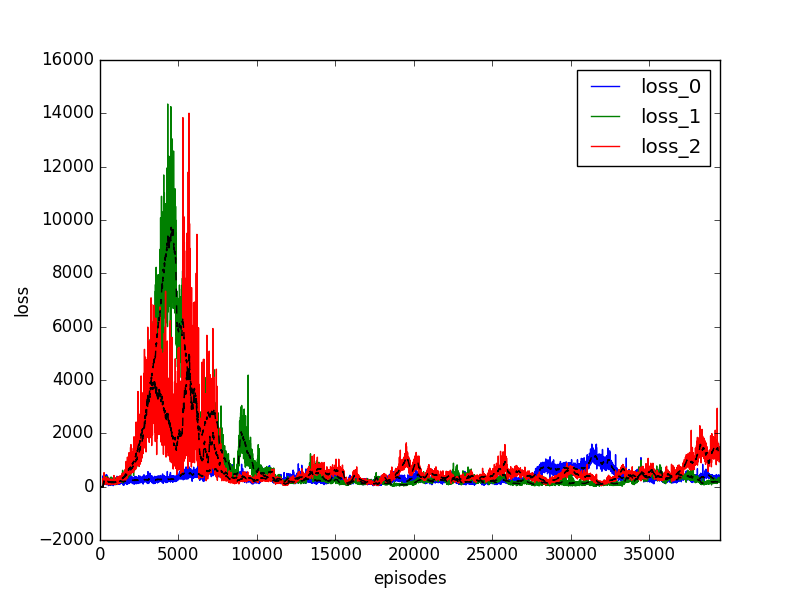
\includegraphics[width=1.5\textwidth]
    {../results/maddpg_2vs1/loss.png}
    \label{fig:maddpg-2vs1-loss}
  \end{subfigure}

  \caption{Plots for steps, average reward, collisions and loss per episode for 1 green vs 2 red agents. \textit{Left Column}: DQN, \textit{Middle Column}: DDPG, \textit{Right Column}: MADDPG}
  \label{fig:2vs1}
\end{figure}
\FloatBarrier
